%!TEX root = ../talk.tex

\section{Introduction}\label{sec:intro}

%%%
\subsection{Background}
%%%

\begin{frame}
  \MyLogo
  \frametitle{Machine learning}  

\begin{itemize}

\item ML gives computers the ability to learn without being explicitly programmed [Samuel 1959]

\item ML explores the study and construction of algorithms that can learn from and make predictions on data

\item Data mining, computational statistics, optimization, ...

\item Fourth paradigm, big data, deep learning, artificial intelligence 

\end{itemize}

\begin{figure}[htbp] %  figure placement: here, top, bottom, or page
   \centering
   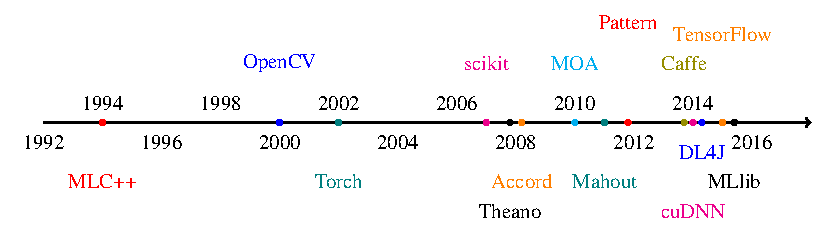
\includegraphics[width=\linewidth]{figures/ML.pdf} 
   \caption{Machine learning packages}
   \label{fig:MLcode}
\end{figure}

\end{frame}

%%%
\subsection{General ML code}
%%%

\begin{frame}
  \MyLogo
  \frametitle{General machine learning code}  

\end{frame}

%%%
\subsection{DL code}
%%%

\begin{frame}
  \MyLogo
  \frametitle{Deep learning}  

\end{frame}

%%%
\subsection{A short introduction on Python}
%%%

\begin{frame}
  \MyLogo
  \frametitle{Python}  

\end{frame}